\documentclass[8pt,xcolor=table,dvipsnames]{beamer}
\usepackage{pgfpages}
\usepackage{yhmath}
\newcommand{\Mod}[1]{\ (\mathrm{mod}\ #1)}
\providecommand{\half}{\frac{1}{2}}
\newcommand{\dg}{^\circ}
\newcommand{\arc}[1]{\wideparen{#1}}
\usetheme{Madrid}

\title{Geometric Transformations III}
\subtitle{UMC K1, 2024}
\author{Nghia Doan}
\institute{MCC Club \& Competitions}
\date{\today}

\begin{document}

\section{Rotations by an Angle}

\begin{frame}[t]
    \frametitle{Geometric Transformations III}
    \framesubtitle{Rotations by an Angle - Example 1}
    \begin{example}
        Three parallel lines $\ell_1$, $\ell_2,$ and $\ell_3$ are given. $A$ is a point on the line $\ell_1$.
        
        \bigbreak
        How can we determine points $B$ and $C$ on $\ell_2$ and $\ell_3$, respectively, such that $ABC$ is an equilateral triangle.
    \end{example}

    \begin{center}
        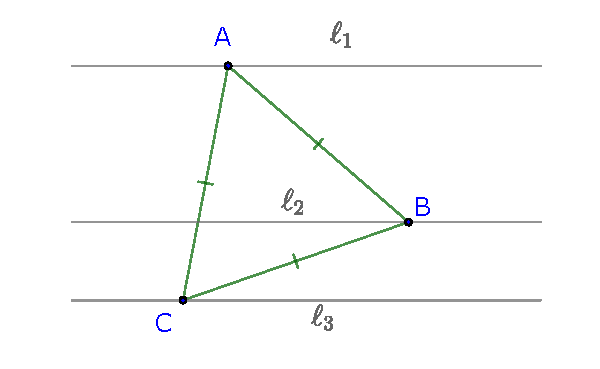
\includegraphics[width=5cm]{./svg/pdf/rotation-4a.pdf}
    \end{center}
\end{frame}

\begin{frame}[t]
    \frametitle{Geometric Transformations III}
    \framesubtitle{Rotations by an Angle - Example 1}
    \begin{overprint}
        \onslide<1>Assume that $\triangle ABC$ is equilateral, then \textbf{a rotation by $60\dg$ about $A$ will carry $B$ to $C$}.
        \begin{center}
            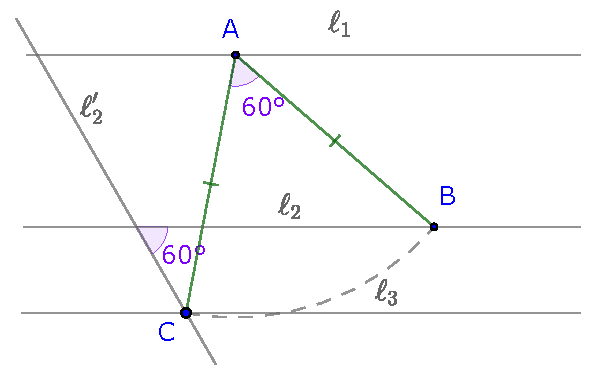
\includegraphics[width=5cm]{./svg/pdf/rotation-4b.pdf}
        \end{center}
        That rotation also carries $\ell_2$  (containing $B$) to $\ell_2'$. The intersection of $\ell_2'$ and $\ell_3$ is $C.$
        \onslide<2>Now we know how to do it. Rotate $\ell_2$ by $60\dg$ about $A$ to obtain $\ell_2'$.
        The intersection of $\ell_2'$ with $\ell_3$ is the position for $C.$
        $B$ can be constructed easily as the intersection of circle centred at $A$ radius $AC.$
        \begin{center}
            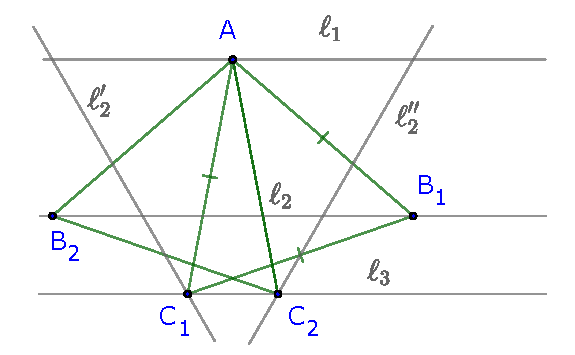
\includegraphics[width=5cm]{./svg/pdf/rotation-4c.pdf}
        \end{center}
    
        \bigbreak
        Note that there are two different solutions (why?)
    \end{overprint}
\end{frame}

\begin{frame}[t]
    \frametitle{Geometric Transformations III}
    \framesubtitle{Rotations by an Angle - Example 2}
    \begin{example}
        Three concentric circles $\omega_1$, $\omega_2,$ and $\omega_3$ are given. $A$ is a point on $\omega_1$.
        
        \bigbreak
        How can we determine points $B$ and $C$ on $\omega_2$ and $\omega_3$, respectively, such that $ABC$ is an equilateral triangle.
    \end{example}

    \begin{center}
        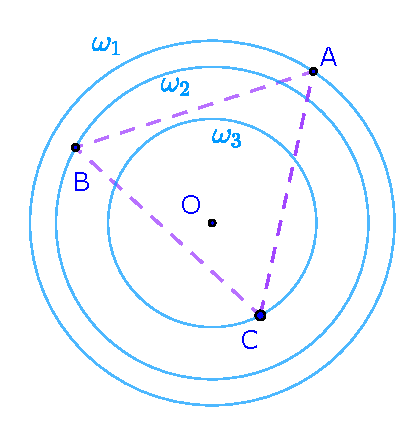
\includegraphics[width=5cm]{./svg/pdf/rotation-5a.pdf}
    \end{center}
\end{frame}

\begin{frame}[t]
    \frametitle{Geometric Transformations III}
    \framesubtitle{Sum of Rotations by an Angle}
    \begin{overprint}
        \onslide<1>Let's take a look at a \textbf{sum of two rotations}:
        \[
            AB \stackrel{\text{rotate}(O_1, \alpha)}{\rightarrow} A_1B_1 \stackrel{\text{rotate}(O_2, \beta)}{\rightarrow} A_2B_2.
        \]
        \begin{center}
            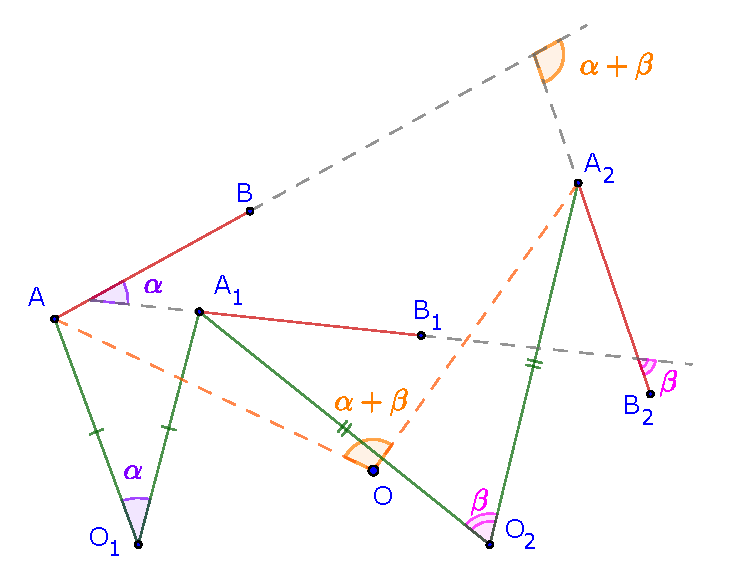
\includegraphics[width=5cm]{./svg/pdf/sum-rotations-1.pdf}
        \end{center}

        It is easy to see that the angle between $A_2B_2$ and $AB$ is $\alpha + \beta$, thus it is a rotation by the angle $\alpha + \beta,$
        We need to determine the position of the center of rotation $O$.
        \onslide<2>Now, what happen with the centers $O_1$ and $O_2$:
        \[
            O_1 \stackrel{\text{rotate}(O_1, \alpha)}{\rightarrow} O_1 \stackrel{\text{rotate}(O_2, \beta)}{\rightarrow} O_1'
            \quad \text{and} \quad O_2'' \stackrel{\text{rotate}(O_1, \alpha)}{\rightarrow} O_2 \stackrel{\text{rotate}(O_2, \beta)}{\rightarrow} O_2.
        \]
        \begin{center}
            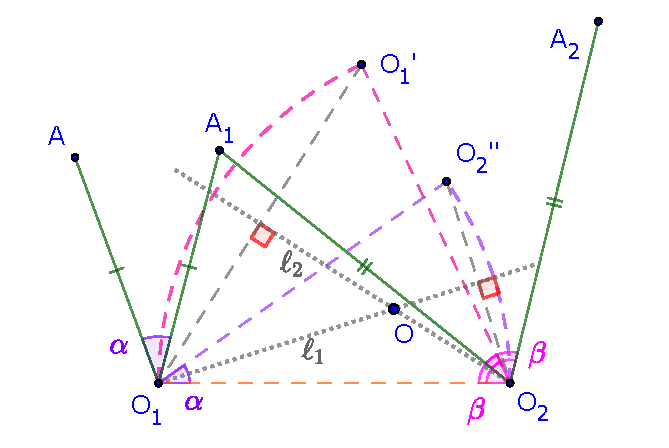
\includegraphics[width=5cm]{./svg/pdf/sum-rotations-2.pdf}
        \end{center}
        Therefore $O$ is on both perpendicular bisectors of $O_1O_1'$ and $O_2''O_2$.

        \bigbreak        
        Hence, $\angle OO_1O_2 = \half \alpha,$  $\angle OO_2O_1 = \half \beta.$
    \end{overprint}
\end{frame}

\begin{frame}[t]
    \frametitle{Geometric Transformations III}
    \framesubtitle{Rotations by an Angle - Example 3}
    Pretty much the same as in the solution for the previous example.
    
    \bigbreak
    Rotate $\omega_2$ by $60\dg$ about $A$ to obtain $\omega_2'$.
    The intersection of $\omega_2'$ with $\omega_3$ is the position for $C.$

    $B$ can be constructed easily as the intersection of circle centred at $A$ radius $AC.$
    \begin{center}
        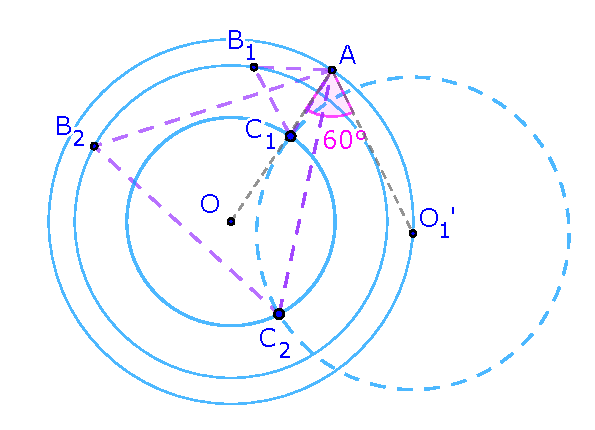
\includegraphics[width=5cm]{./svg/pdf/rotation-5b.pdf}
    \end{center}

    \bigbreak
    Note that there are \textbf{at most four} different solutions (why?).
\end{frame}

\begin{frame}[t]
    \frametitle{Geometric Transformations III}
    \framesubtitle{Rotations by an Angle - Example 4}
    \begin{example}
        Let $E$ be a point in the square $ABCD$ such that $\angle EAB = \angle EBA = 15\dg.$
        Prove that $\triangle CDE$ is equilateral.
    \end{example}
    \begin{overprint}
        \onslide<1>\begin{center}
            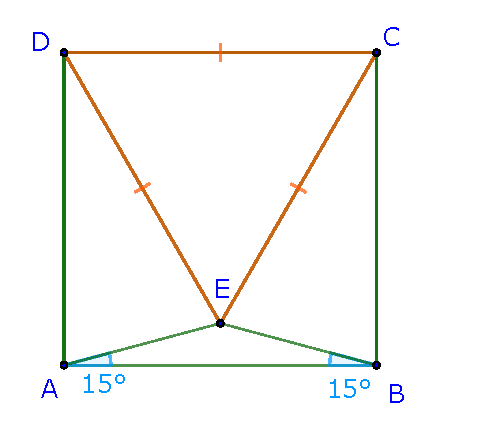
\includegraphics[width=4cm]{./svg/pdf/rotation-11-2.pdf}
        \end{center}
        \onslide<2->\begin{center}
            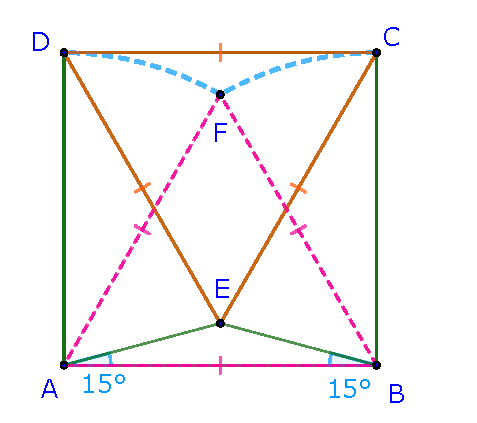
\includegraphics[width=4cm]{./svg/pdf/rotation-11.pdf}
        \end{center}
    \end{overprint}
    \onslide<2->Let $F$ be a point inside $ABCD$ such that $\triangle ABF$ is equilateral.
    \bigbreak
    \onslide<3->The rotation about $A$ by $30\dg$ clockwise sends $D$ to $F$,
    and the rotation about $B$ by $30\dg$ clockwise sends $F$ to $C$.
    \bigbreak
    \onslide<4->Thus the sum of rotation is a rotation about $O$ by $60\dg$ sends $D$ to $C$, where
    $O$ is the point such that $OC = OD,$ $\angle DOC = 60\dg,$ and $\angle OAB = OBA = 15\dg.$
    \onslide<5->Hence, $O \equiv E.$
\end{frame}

\begin{frame}[t]
    \frametitle{Geometric Transformations III}
    \framesubtitle{Rotations by an Angle - Example 5}
    \begin{example}
        Let $ABGF$ and $ACDE$ be squares outside $\triangle ABC.$ Let $H$ be the midpoint of $DG$. 
        Show that $HB = HC$ and $HB \perp HC.$
    \end{example}

    \begin{center}
        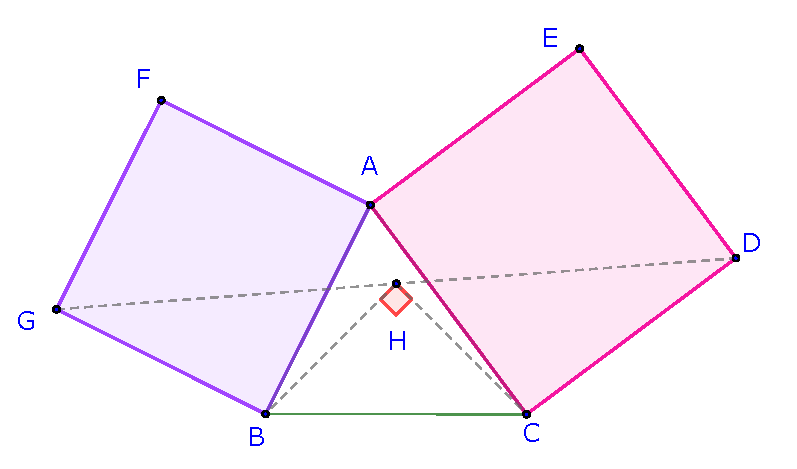
\includegraphics[width=5cm]{./svg/pdf/rotation-10.pdf}
    \end{center}
    \onslide<2->Since $CD = CA$ and $\angle DCA = 90\dg$, so the rotation about $C$ by $90\dg$ anti-clockwise sends $D$ to $A$.
    Also, the rotation about $B$ by $90\dg$ anti-clockwise sends $A$ to $G$.
    \bigbreak
    \onslide<3->Thus the sum of rotation is a rotation about $O$ by $180\dg$ sends $D$ to $G$, where
    $O$ is the point such that $\angle OCB = 45\dg$ and $\angle OBC = 45\dg.$
    \bigbreak
    \onslide<4->A rotation of about $O$ by $180\dg$ sends $D$ to $G$ means that $OD = OG$, thus $O \equiv H.$
\end{frame}

\begin{frame}[t]
    \frametitle{Geometric Transformations III}
    \framesubtitle{Rotations by an Angle - Example 6}
    \begin{example}
        On the sides of an arbitrary triangle $ABC,$ exterior to it, construct isosceles triangles $BCA_1$ $ACB_1$, $CAB_1$
        with angles at the vertices $A_1$, $B_1$, and $C_1$, respectively equal to $\alpha$, $\beta$ and $\gamma$.
        \bigbreak
        Prove that if $\alpha + \beta + \gamma = 360\dg$, then the angles of the triangle $A_1B_1C_1$
        are equal to $\half\alpha$, $\half\beta$ and $\half\gamma$, that is, they do not depend on the shape of the triangle $ABC.$
    \end{example}

    \begin{center}
        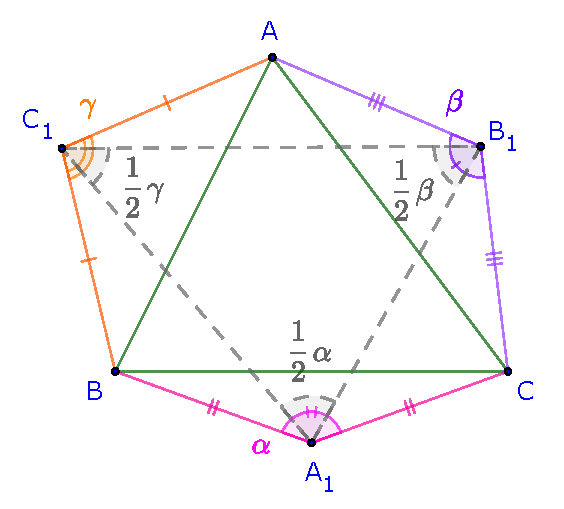
\includegraphics[width=5cm]{./svg/pdf/rotation-6a.pdf}
    \end{center}
\end{frame}

\begin{frame}[t]
    \frametitle{Geometric Transformations III}
    \framesubtitle{Rotations by an Angle - Example 6}
    \begin{overprint}
        \onslide<1>First, point $A$ is taken into itself by the sum of three rotations through the angles $\beta$, $\alpha$, and $\gamma$
        ($\alpha + \beta + \gamma = 360\dg$) about the centers $B_1, A_1, C_1$:
        \[
            A \stackrel{\text{rotate}(B_1, \beta)}{\rightarrow} C \stackrel{\text{rotate}(A_1, \alpha)}{\rightarrow} B 
            \stackrel{\text{rotate}(C_1, \gamma)}{\rightarrow} A. 
        \]
        \begin{center}
            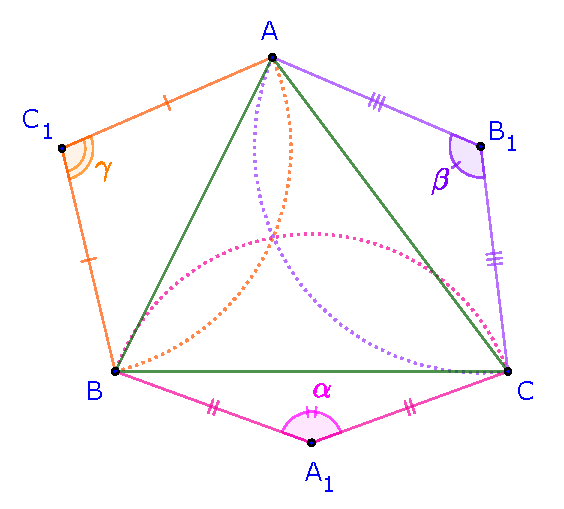
\includegraphics[width=5cm]{./svg/pdf/rotation-6b.pdf}
        \end{center}
        Thus, the \textbf{sum of the these rotations} is the \textbf{identity transformation}.
        \onslide<2>Let $C'$ be the center of the rotation equivalent to the sum of the rotations about $B_1$ and $A_1$.
        Then it is the rotation through $\alpha + \beta = 360\dg - \gamma$ brings $A$ to $B$.
        \bigbreak
        However, the rotation about $C_1$ through $\gamma$ brings $A$ to $B$ in opposite direction.
        Since a rotation through an angle $\theta$ is the same as the rotation through an angle $360\dg - \theta$
        about the same center in the opposite direction, thus $C_1 \equiv C'.$
        \begin{center}
            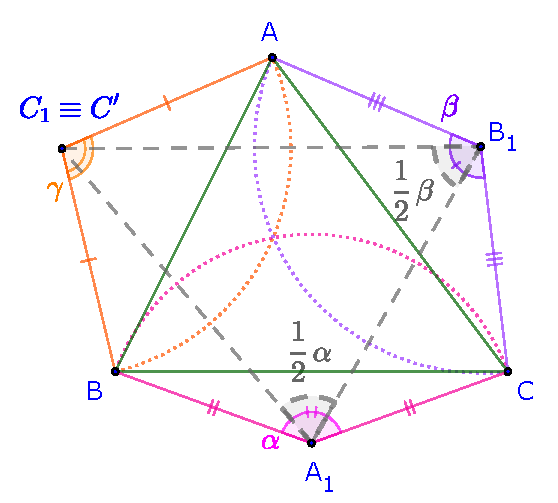
\includegraphics[width=5cm]{./svg/pdf/rotation-6c.pdf}
        \end{center}
        Therefore $\angle C_1A_1B_1 = \half \alpha, \angle C_1B_1A_1 = \half \beta,$ and similarly $\angle B_1C_1A_1 = \half \gamma.$ 
    \end{overprint}
\end{frame}

\begin{frame}[t]
    \frametitle{Geometric Transformations III}
    \framesubtitle{Rotations by an Angle - Example 7}
    \begin{example}
        In triangle $ABC$, the angle bisector at vertex $C$ intersects the circumcircle
        and the perpendicular bisectors of sides $BC$ and $CA$ at points $R$, $P$, and $Q$, respectively.
        The midpoints of $BC$ and $CA$ are $K$ and $L$, respectively.
        \bigbreak
        Prove that triangles $RPK$ and $RQL$ have the same area.
    \end{example}

    \begin{center}
        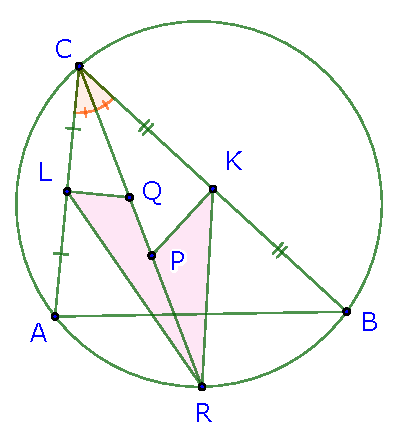
\includegraphics[width=4.5cm]{./svg/pdf/imo-2007-4.pdf}
    \end{center}
\end{frame}

\begin{frame}[t]
    \frametitle{Geometric Transformations III}
    \framesubtitle{Rotations by an Angle - Example 7}
    \begin{overprint}
        \onslide<1>WLOG, assume $AC<BC$. Let $ACB=\gamma$.
        From the right triangles $CLQ$ and $CKP$, 
        \[
            \angle OPQ=\angle OQP=90\dg - \frac{\gamma}{2}.
        \]
        Thus, $OPQ$ is isosceles, $OP=OQ$, and $\angle POQ=180\dg - 2\left(90\dg - \frac{\gamma}{2}\right)= \gamma$.
        \begin{center}
            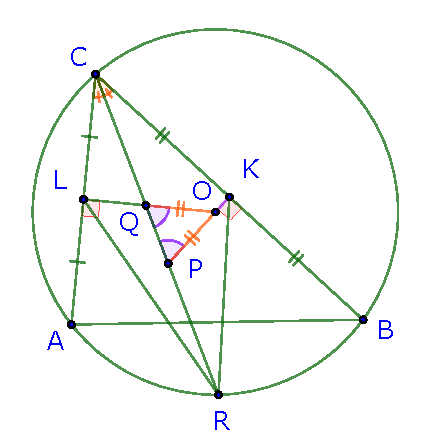
\includegraphics[width=4.5cm]{./svg/pdf/imo-2007-4-2.pdf}
        \end{center}
        \onslide<2>$CR$ is the angle bisector, so $R$ is midpoint of $\arc{AB}$, and 
        \[
            \angle ROA=\angle ROB=\gamma,\ AR = RB.
        \]
        \begin{center}
            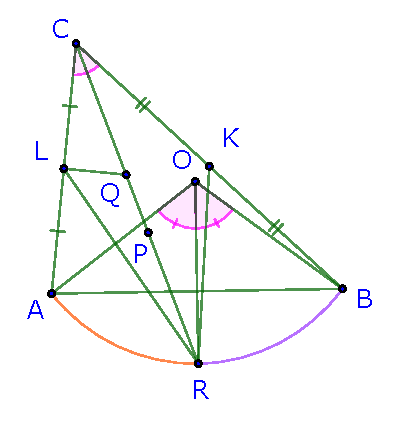
\includegraphics[width=4.5cm]{./svg/pdf/imo-2007-4-3.pdf}
        \end{center}
        \onslide<3>Consider the \textbf{rotation around $O$ by angle $\gamma$}, see the figure below.
        This transformation moves:
        \[
            Q \rightarrow P,\ A \rightarrow R,\ R \rightarrow B \Rightarrow \triangle QAR \cong \triangle PRB \Rightarrow [QAR] = [PRB].
        \]
        \begin{center}
            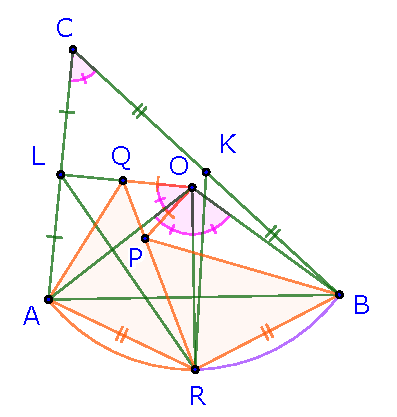
\includegraphics[width=4.5cm]{./svg/pdf/imo-2007-4-4.pdf}
        \end{center}
        \onslide<4>Finally:
        \[
            \frac{[RQL]}{[RQA]}=\frac{\text{distance}(L,CR)}{\text{distance}(A,CR)}=\frac{CL}{CA}=\frac{1}{2},\
            \text{and similarly}\ \frac{[RPK]}{[BPR]} = \frac{1}{2} 
        \]
        Therefore,
        \[
            [RQL]=\half [RQA]=\half [BPR]=[RPK]
        \]
        \begin{center}
            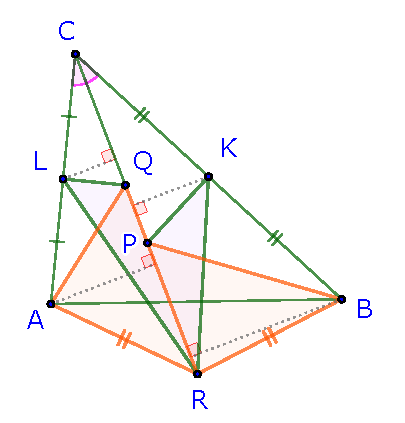
\includegraphics[width=4.5cm]{./svg/pdf/imo-2007-4-5.pdf}
        \end{center}
    \end{overprint}
\end{frame}

\begin{frame}[t]
    \frametitle{Geometric Transformations III}
    \framesubtitle{Symmetry - Example 1}
    \begin{example}
        $\angle MON$ is given, together with two points $A$ and $B$.
        Find a point $X$ on the side $OM$ such that the triangle $XYZ$ is isosceles: $XY = XZ$, 
        where $Y$ and $Z$ are on the points of intersection of $XA$ and $XB$ with $ON.$ 
    \end{example}

    \begin{center}
        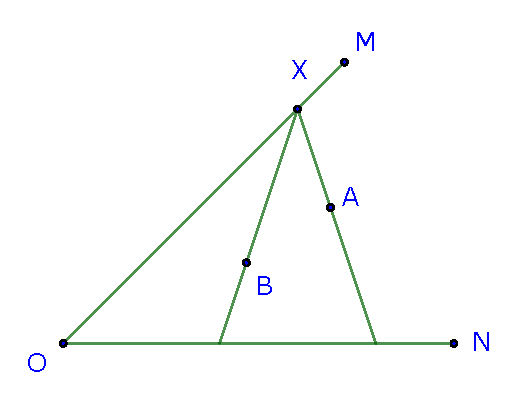
\includegraphics[width=5cm]{./svg/pdf/symmetry-1a.pdf}
    \end{center}
\end{frame}

\begin{frame}[t]
    \frametitle{Geometric Transformations III}
    \framesubtitle{Symmetry - Example 1}
    \begin{center}
        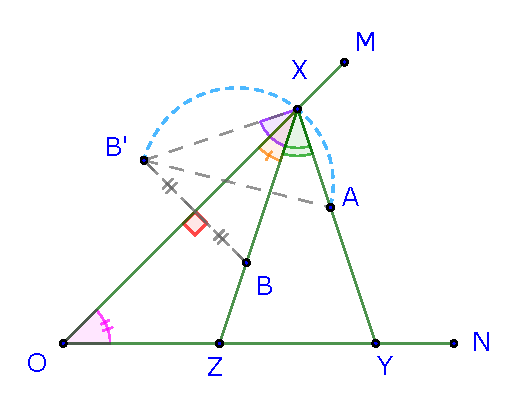
\includegraphics[width=5cm]{./svg/pdf/symmetry-1b.pdf}
    \end{center}
    Let $B'$ be the image of $B$ over $OM,$ \onslide<2->then:
    \[
        \angle B'XA = \angle B'XB + \angle YXZ,\  \onslide<3->\angle B'XB = 2\angle OXZ = 2(\angle XZY - \angle MON)
        \onslide<4->\Rightarrow \angle B'XA = 180\dg - 2\angle MON.
    \]

    \onslide<5->Thus, $X$ is the intersection of $OM$ with the arc constructed on the chord $AB',$ that subtends an angle equal to $180\dg - 2\angle MON.$
\end{frame}

\begin{frame}[t]
    \frametitle{Geometric Transformations III}
    \framesubtitle{Symmetry - Example 2}
    \begin{example}
        Construct a quadrilateral $ABCD$ in which a circle can be inscribed,
        given the lengths of two adjacent sides $AB$ and $AD$ and the angles at the vertices $B$ and $D.$
    \end{example}

    \begin{center}
        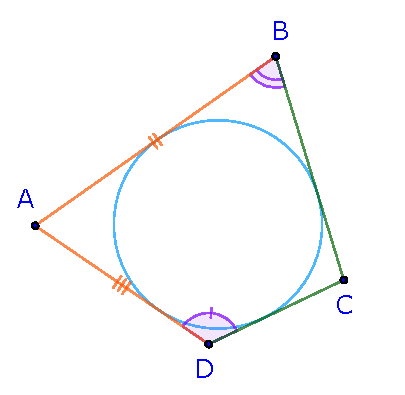
\includegraphics[width=5cm]{./svg/pdf/symmetry-2a.pdf}
    \end{center}
\end{frame}

\begin{frame}[t]
    \frametitle{Geometric Transformations III}
    \framesubtitle{Symmetry - Example 2}
    \begin{overprint}
        \onslide<1>The key idea here is that the reflection of $CD$ over the line through $A$ and the center of the circle is a tangent to the circle!
        \begin{center}
            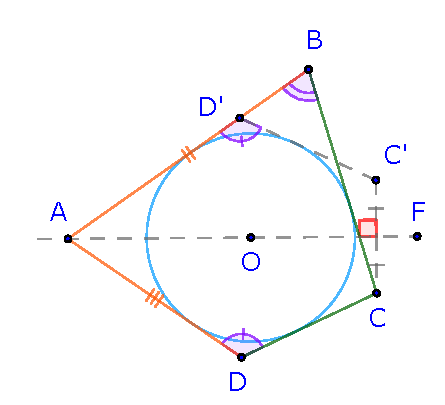
\includegraphics[width=5cm]{./svg/pdf/symmetry-2d.pdf}
        \end{center}
        \onslide<2>First, we start the construction by point $A$ then segment $AB$,
        then segment $AD_1 = AD$ where $D$ is on the line $AB,$ same side as $B$ in respect to $A$.

        \bigbreak
        Second, because $\angle B$ and $\angle D_1= \angle D$ are known, thus we can construct rays going from $B$ and $D_1.$
        
        \bigbreak
        Finally, we construct a circle tangents to all three lines.
        \begin{center}
            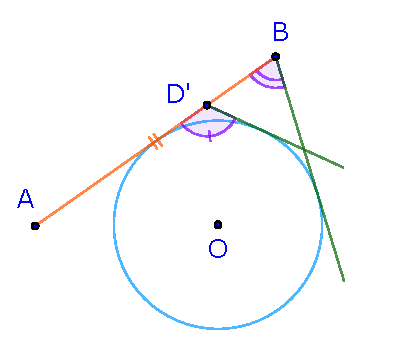
\includegraphics[width=5cm]{./svg/pdf/symmetry-2b.pdf}
        \end{center}
        \onslide<3>The rest is simple, we reflect $D'$ and its ray over the line $AO$ where $O$ is the center of the circle.
        The reflected ray will intersect the ray from $B$ at $C.$ We are done.
        \begin{center}
            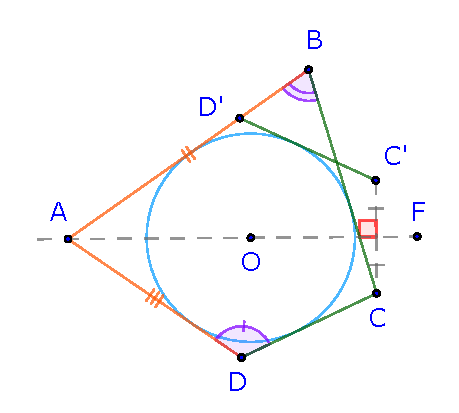
\includegraphics[width=5cm]{./svg/pdf/symmetry-2c.pdf}
        \end{center}
    \end{overprint}
\end{frame}

\begin{frame}[t]
    \frametitle{Geometric Transformations III}
    \framesubtitle{Symmetry - Example 3}
    \begin{example}
        \textit{A billiard ball bounces off a side of a billiard table in such a manner that the two lines along
        which it moves before and after hitting the sides are equally inclined to the side.}

        Suppose a billiard table were bordered by $n$ lines $\ell_1, \ell_2, \ldots, \ell_n$.
        Let $A$ and $B$ be two given points on the billiard table.
        In what direction should one hit a ball placed at $A$
        so that it will bounce consecutively off the lines $\ell_1, \ell_2, \ldots, \ell_n$,
        and then pass through the point $B$ (see the diagram below, where $n = 3$)?
    \end{example}

    \begin{center}
        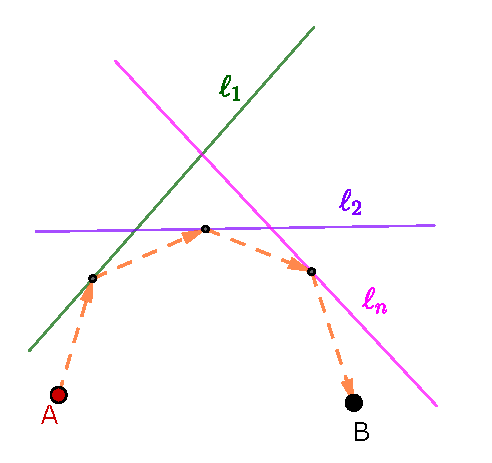
\includegraphics[width=4cm]{./svg/pdf/symmetry-3a.pdf}
    \end{center}
\end{frame}

\begin{frame}[t]
    \frametitle{Geometric Transformations III}
    \framesubtitle{Symmetry - Example 3}
    Assume that the problem has been solved, that is, that points
    $X_1, X_2, \ldots X_n$ have been found on the lines $\ell_1, \ell_2, \ldots, \ell_n$ such that
    $A X_1 X_2 \cdots X_n B$ is the path of a billiard ball (the case $n = 3$).
    \begin{center}
        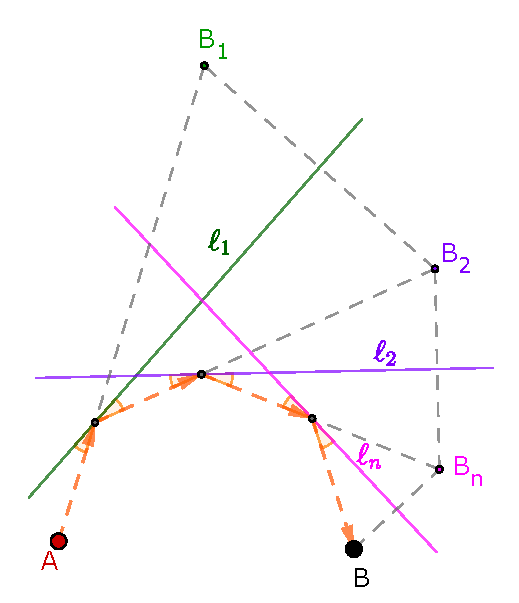
\includegraphics[width=3.5cm]{./svg/pdf/symmetry-3b.pdf}
    \end{center}
    \begin{overprint}
        \onslide<1>It is easy to see that the point $X_n$, is the point of intersection of the line $\ell_n$ with the line $X_{n-1}B_n$,
        where $B_n$, is the image of $B$ in $\ell_n$, that is, the points $B_n$,$X_n$, $X_{n-1}$ lie on a line.
        \bigbreak
        But then the point $X_{n-1}$ is the point of intersection of the line $\ell_{n-1}$ with the $X_{n-2}B_{n-1}$,
        where $B_{n-1}$, is the image of $B_n$ in $\ell_{n-1}$ and so on.
        \onslide<2>Here's the construction: Reflect the point $B$ in $l_n$, obtaining the point $B_n$;
        next reflect $B_n$ in $l_{n-1}$ to obtain $B_{n-1},$ and so forth, until the image $B_1$ of the point $B_2$, in line $\ell_1$ is obtained.
        \bigbreak
        The point $X_1$, that determines the direction in which the billiard ball at $A$ must be hit,
        is obtained as the point of intersection of the line $\ell_1$ with the line $AB_1$.
        It is then easy to find the points $X_2, \ldots X_n$ with the aid of the points $B_2, \ldots B_n$ and $X_1$.
    \end{overprint}
\end{frame}

\begin{frame}[t]
    \frametitle{Geometric Transformations III}
    \framesubtitle{Symmetry - Example 4}
    \begin{example}
        A \textit{center of symmetry} of a set $S$ means a point $O,$ not necessarily in $S,$ such that for every point $A \in S,$
        there is another point $B \in S$ such that $O$ is the midpoint of $AB.$ We say that $B$ is symmetric to $A$ with respect to $O.$
        \bigbreak
        Prove that a set $S$ containing a \textit{finite} number of points cannot have more than one center of symmetry.
    \end{example}
    \bigbreak
    Example from Geometric Transformations II session:
    \bigbreak
    \textit{The strip formed by two parallel lines clearly has infinitely many centers of symmetry.
    Can a figure have more than one, but only a finite number of centers of symmetry (for example, can it have two and only two centers of symmetry)?}
    \begin{center}
        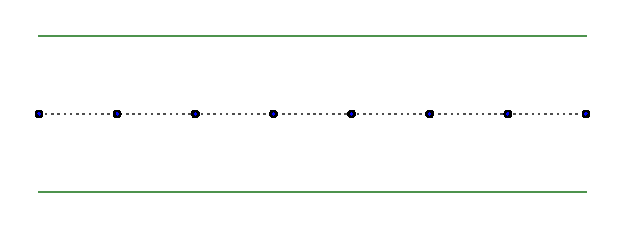
\includegraphics[width=5cm]{./svg/pdf/rotation-9.pdf}
    \end{center}
\end{frame}

\begin{frame}[t]
    \frametitle{Geometric Transformations III}
    \framesubtitle{Symmetry - Example 4 - Solution by the Extremal Principle}
    \begin{overprint}
        \onslide<1>Let $O$ be the center of symmetry. Suppose to the contrary that $\mathcal{F}$ has another center of symmetry $O' \not \equiv O.$
        Since $\mathcal{F}$ contains a finite number of points, by the Extremal Principle,
        \textbf{there exists $A \in \mathcal{F}$ with the greatest distance from $O$}.
        We consider two cases $A, O, O'$ are collinear and $A, O, O'$ are not collinear.

        \textbf{Case 1:} $A, O, O'$ are collinear. There are three sub-cases.

        \textbf{Case 1.1:} $O$ is between $A$ and $O'.$ Let $X$ be the point symmetric to $A$ with respect to $O'$
        (see the diagram below on the left).
        Then $XO > XO' = AO' > AO,$ which is a contradiction to the maximality of $AO.$
        \begin{center}
            \includegraphics[width=12cm]{../Learning-Problem-Solving-2nd-Edition/svg/pdf/24-25-s1-g4-p13.pdf}
        \end{center}
        \textbf{Case 1.2:} $O'$ is between $A$ and $O.$ Let $Y$ be the point symmetric to $A$ with respect to $O,$
        and let $Y'$ be the point symmetric to $Y$ with respect to $O'$ (see the diagram above on the right).
        Then $Y'O > Y'O' = YO' > YO = AO,$ which is a contradiction to the maximality of $AO.$

        \textbf{Case 1.3:} $A$ is between $O$ and $O'.$ Let $Z$ be the point symmetric to $A$ with respect to $O'$
        (see the diagram below) Then $ZO > AO,$ which is a contradiction to the maximality of $AO.$
        \begin{center}
            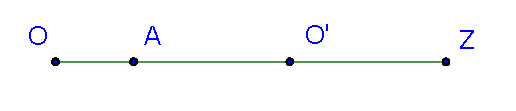
\includegraphics[width=5cm]{./svg/pdf/24-25-s1-g4-p13-2.pdf}
        \end{center}
        \onslide<2>\textbf{Case 2:} $A, O, O'$ are not collinear.
        Let $B$ be the point symmetric to $A$ with respect to $O,$ let $A'$ the point symmetric to $A$ with respect to $O',$
        and let $B'$ the point symmetric to $B$ with respect to $O'$ (see the diagram below).
        \begin{center}
            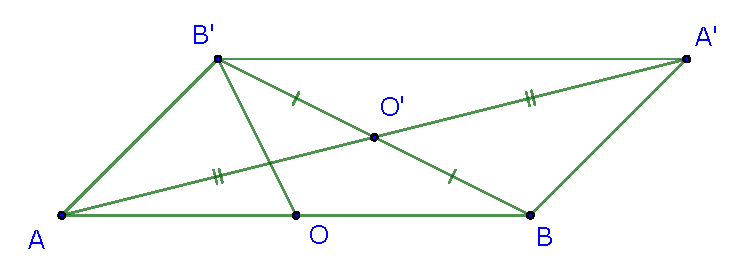
\includegraphics[width=7cm]{./svg/pdf/24-25-s1-g4-p13-3.pdf}
        \end{center}
        Because the quadrilateral $ABA'B'$ has 2 diagonals that bisect each other ($AO'=O'A', BO'=O'B'$), thus $ABA'B'$ is a parallelogram.
        Therefore $\angle B'AB + \angle A'BA = 180\dg,$ so one of $\angle B'AB$ and $\angle A'BA$ is greater than or equal to $90\dg.$
    
        \textbf{Case 2.1:} $\angle A'BA \ge 90\dg,$ then $A'O > BO = AO$ (because $\angle A'BO$ is the largest angle in $\triangle A'BO$),
        which is a contradiction to the maximality of $AO.$
    
        \textbf{Case 2.2:} $\angle B'AB \ge 90\dg,$ then $B'O > AO$ (because $\angle B'AO$ is the largest angle in $\triangle B'AO$),
        which is a contradiction to the maximality of $AO.$
    
        \bigbreak
        Hence, $\mathcal{F}$ cannot have more than one center of symmetry.
    \end{overprint}
\end{frame}

\begin{frame}[t]
    \frametitle{Geometric Transformations III}
    \framesubtitle{Vector Introduction}
    \begin{overprint}
        \onslide<1>\begin{definition}[Vector]
            Vector is a \textit{directed line segment,} or as an arrow connecting an initial point A with a terminal point B, and denoted by $\overrightarrow{AB}.$
            Vectors are usually denoted in lowercase boldface, as in $\textbf{u}, \textbf{v},$ or $\textbf{w}.$
            \bigbreak
            A vector is called \textit{zero vector} if the initial point and the terminal point are the same, in other words its magnitude is 0.
            A zero vector has an arbitrary or indeterminate direction.
            A \textit{unit vector} is any vector with a length of one.
        \end{definition}
        
        \onslide<2>\begin{definition}[Equality]
            Two vectors are said to be \textit{equal} if they have the same magnitude and direction.
        
            The equality of $\textbf{u}, \textbf{v}$ is denoted as $\textbf{u} = \textbf{v}.$
        \end{definition}
        
        \onslide<3>\begin{definition}[Parallel, Opposite, and Antiparallel]
            Two vectors are \textit{parallel} if they have the same direction but not necessarily the same magnitude: 
            $\overrightarrow{AB}$ and $\overrightarrow{A_1B_1}$ ($\overrightarrow{AB} \parallel \overrightarrow{A_1B_1}$)
            or $\overrightarrow{AB}$ and $\overrightarrow{A_3B_3}$ ($\overrightarrow{AB} \parallel \overrightarrow{A_3B_3}.$)
        
            Two vectors are \textit{opposite} if they have the same magnitude but opposite direction: $\overrightarrow{AB}$ and $\overrightarrow{A_2B_2}$
        
            Two vectors are \textit{antiparallel} if they have opposite direction: $\overrightarrow{A_2B_2}$ and $\overrightarrow{A_3B_3}.$
        \end{definition}
        
        \onslide<4>\begin{definition}[Addition and Subtraction]
            The \textit{sum} of $\textbf{u}$ and $\textbf{v}$ of two vectors may be defined as $\textbf{u} + \textbf{v}.$
            The resulting vector is sometimes called the resultant vector of $\textbf{u}$ and $\textbf{v}$.
            
            The addition may be represented graphically by placing the tail of the arrow $\textbf{v}$ at the head of the arrow $\textbf{u}$,
            and then drawing an arrow from the tail of $\textbf{u}$ to the head of $\textbf{v}$.
            The new arrow drawn represents the vector $\textbf{u} + \textbf{v}$, shown as below.
        
            The \textit{difference} of $\textbf{u}$ and $\textbf{v}$ is $\textbf{u} - \textbf{v},$ or $\textbf{u} + (-\textbf{v}),$ 
            which is the addition of $\textbf{u}$ to the opposite of $\textbf{v}.$
        \end{definition}
    \end{overprint}
    \begin{center}
        \includegraphics[width=9cm]{../Learning-Problem-Solving-2nd-Edition/svg/pdf/24-25-s1-g4-t1.pdf}
    \end{center}
\end{frame}

\begin{frame}[t]
    \frametitle{Geometric Transformations III}
    \framesubtitle{Symmetry - Example 4 - Solution by Vectors}
    \onslide<1->Suppose that there were two centers of symmetry, $P$ and $Q.$ Let $S$ be a set of pairwise distinct points in $\mathcal{F}$:
    \[ S = \{A_1,A_2, \ldots, A_n\}. \]
    \bigbreak
    \onslide<2->For each $k = 1,2, \ldots, n,$ let $B_k$ denotes the point in $S$ that is symmetric to $A_k$ with respect to $P.$
    \bigbreak
    \onslide<3->By the definition of symmetry, we have $\overrightarrow{PA_k} + \overrightarrow{PB_k} = \textbf{0}.$
    \bigbreak
    Note that for each $k \in \{1,2, \ldots, n\}$, there exists $j\in \{1,2, \ldots, n\}$ $B_k = A_j.$
    So $(B_1, B_2,\ldots, B_n)$ is a permutation of $(A_1, A_2,\ldots, A_n).$
    \bigbreak
    \onslide<4->Summing this from $k = 1$ to $k = n$ implies that:
    \[ 
        \sum_{k=1}^{n} \overrightarrow{PA_k} + \overrightarrow{PB_k} = \textbf{0},\ 
        \sum_{k=1}^{n} \overrightarrow{PA_k} = \sum_{k=1}^{n} \overrightarrow{PB_k}
        \Rightarrow \sum_{k=1}^{n} \overrightarrow{PA_k} = \textbf{0}.
    \]
    \onslide<5->By the same reasoning, we also have $\overrightarrow{QA_1} + \overrightarrow{QA_2} + \ldots + \overrightarrow{QA_n} = \textbf{0}.$
    Subtracting, 
    \[ 
        \textbf{0} = \sum_{k=1}^{n}  \overrightarrow{PA_k} -  \sum_{k=1}^{n} \overrightarrow{QA_k} = n\overrightarrow{QP} 
        \Rightarrow \overrightarrow{QP} = 0 \Rightarrow \boxed{Q \equiv P.}
    \]
\end{frame}

\end{document}
